\documentclass[acmlarge]{acmart}

\usepackage{booktabs} % For formal tables


\usepackage[ruled]{algorithm2e} % For algorithms
\renewcommand{\algorithmcfname}{ALGORITHM}
\SetAlFnt{\small}
\SetAlCapFnt{\small}
\SetAlCapNameFnt{\small}
\SetAlCapHSkip{0pt}
\IncMargin{-\parindent}
\newcommand{\Mod}[1]{\ (\mathrm{mod}\ #1)}
\usepackage{fancyvrb}
% Metadata Information
%\acmJournal{PACMHCI}
%\acmVolume{9}
%\acmNumber{4}
%\acmArticle{39}
%\acmYear{2010}
%\acmMonth{3}
%\acmArticleSeq{11}


% DOI
\acmDOI{0000001.0000001}

% Paper history
%\received{February 2007}
%\received{March 2009}
%\received[accepted]{June 2009}


% Document starts
\begin{document}
% Title portion
\title{Security Suite: Team 4 EECS 444 Final Project}
% \titlenote{We can add a note to the title}

\author{Kim Almcrantz}
%\affiliation{\institution{Case Western Reserve University}}
\email{kaa97@case.edu}

\author{Mark Lalor}
%\affiliation{\institution{Case Western Reserve University}}
\email{mwl58@case.edu}

\author{Brian Li}
%\affiliation{\institution{Case Western Reserve University}}
\email{bvl8@case.edu}

\author{Vanessa Melikian}
%\affiliation{\institution{Case Western Reserve University}}
\email{vlm21@case.edu}

\author{Maya Nayak}
%\affiliation{\institution{Case Western Reserve University}}
\email{mkn30@case.edu}

\author{Jacob Wise}
%\affiliation{\institution{Case Western Reserve University}}
\email{jsw107@case.edu}

\keywords{encryption, cipher, hash, entropy}

\maketitle

% The default list of authors is too long for headers.
% \renewcommand{\shortauthors}{G. Zhou et al.}

\section{Abstract}
Sensitive data such as bank details, and personal information is continuously exchanged over the Internet. In an attempt to fend off malicious users attempting to gain access to this data, digital information must be made hidden. A common way to do this is through encryption. In particular, cryptography offers many techniques to encrypt data. Each technique faces tradeoffs and operates best given certain assumptions. In this paper, we aim to explain and implement the following cryptographic techniques: RSA, DES, and Vigen\`{e}re Cipher. In addition to explanations and implementations of these encryption techniques, we will also present tools that crack the Vignere and MD5 hash algorithm. With these tools, we hope to illustrate that some cryptographic techniques have vulnerabilities that can be exploited by ill-intentioned users.


\section{Introduction}\label{sec:intro}

Modern communications require special methods to ensure the confidentiality of information in the presence of adversaries that want to intercept or maliciously modify communicated data. An adversary may try to compromise the confidentiality of data or bypass an authentication altogether with a carefully-crafted message.

This article is divided into several sections, in Section [\ref{sec:intro}], we introduce the cryptographic environment that we will explore. In Section [\ref{sec:algorithms}] we describe implementations of several symmetric and asymmetric encryption algorithms, and then Section [\ref{sec:gui}] we present our tool \textsc{SecuritySuiteGUI}, a software suite to experiment with these implementations. We then demonstrate the power of password cracking with a hashcat demo in Section [\ref{sec:hashcat}]. Finally, we demonstrate how the Vigen\`{e}re cipher may be easily cracked with computational power in Section [\ref{sec:vinegar}]. We evaluate our methods in Section [\ref{sec:evaluation}], and then discuss our techniques, challenges, and other thoughts in Section [\ref{sec:discussion}]. Finally, we discuss our final conclusions in Section [\ref{sec:conclusions}].

\subsection{Overview of Cryptography Algorithms}
\subsubsection{DES}
\hspace*{\fill} \\ % force newline
Data Encryption Standard (DES) is a type of data encryption described as a symmetric-key block cipher. A symmetric key uses the same key to encrypt and decrypt a message, which means that both the sending and receiving side of the transaction must use the same private key. A block cipher takes in a string of bits and transforms it through bit-wise operations into a new string of bits with the same length. 

DES begins by taking in two 64-bit inputs: a key and message. In general, all operations are done at the bit-level, using tables of predetermined size and content. The algorithm then permutes the input key according to a given table, PC-1. This results in a new 56-bit key. The new key is then split into two 28-bit halves, $C_{0}$ and $D_{0}$. Using these halves, we iterate 16 times to create 16 sets of blocks (n from 1 to 16). Every $C_{n}$ and  $D_{n}$ is computed by performing a set number of left shifts (either one or two) on $C_{n-1}$ and $D_{n-1}$.
 The resulting pairs are concatenated into a 56-bit $C_{n}D_{n}$, and permuted with the table PC-2 to form 16 keys, $K_{n}$. At this point, we have the 16 sub-keys (of size 48 bits) necessary. 

Moving to the encryption of the message itself, we begin by permuting it with the table IP. The resulting permutation is then split into 32-bit halves, $L_{0}$ and $R_{0}$. Over the course of 16 iterations, we create 16  sets of blocks using the Feistel function f:
$L_{n} = R_{n-1}$
$R_{n} = L_{n-1} \bigoplus f(R_{n-1}, K_{n})$ 
	The Feistel function involves taking in a subkey $K_{n}$ and block $R_{n - 1}$. It permutes $R_{n - 1}$ using table E, and then XORs the result with $K_{n}$. It then takes the resulting block and permutes it using a series of 8 S-boxes. There is then a final permutation on the S-box output with table P. At the end of the iterations we are left with a concatenated block, $R_{16}L_{16}$. This block is finally permuted with a table $IP^{-1}$, and returned as the output of the DES algorithm. Note that encryption and decryption are almost exactly the same, except for the order in which the subkeys are applied. For encryption, the keys are applied $K_{1}$ to $K_{16}$ and for decryption they are applied $K_{16}$ to $K_{1}$.

While DES used to be heavily adopted, due to the small size of the key it has been found to be insecure by a brute force attack. It is no longer used as a standard. Though Triple DES, an extension of DES, is thought to be secure, its implementation is out of the scope of this paper. 

\subsubsection{RSA}
\hspace*{\fill} \\ % force newline
Unlike DES and Vignere, RSA is an asymmetric cipher. Specifically, this means that the RSA cipher (i.e. public key) used to encrypt a message cannot be used to decrypt the the encrypted message whereas the cipher used to encrypt a message in DES and Vignere can be used to decrypt the encrypted message by reversing the encryption process.
		
To use RSA, a user first generates a key pair. The key pair contains a private key, public key, and a public key exponent. The public key and public key exponent can be made public so that other users can send the original user an encrypted message. The original user can use his/her private key to decrypt messages encrypted with the published public key and exponent. The main benefit that asymmetric encryption provides is that communicating entities can securely communicate without exchanging a decryption key/cipher.

The key mechanic in RSA comes from the following congruence:

\begin{equation}
\label{rsa_mechanic}
	m^{ed} \equiv m \Mod{pq}
\end{equation}

When $ed$ satisfies:

\begin{equation}
\label{ed_equiv}
	ed \equiv 1 \Mod{\lambda(pq)}
\end{equation}
\begin{equation}
\label{carmichael}
	\lambda(pq) = lcm(p - 1, q - 1)
\end{equation}

To see why \ref{rsa_mechanic} is true, we will give a proof:
\begin{equation}
\label{rsa_proof}
\begin{split}
	m^{ed} 
	\equiv m^{k\lambda(pq) + 1} \Mod{pq} \\
	\equiv m \times m^{k\lambda(pq)} \Mod{pq} \\
	\equiv m \times (m^{\lambda(pq)})^{k} \Mod{pq} \\
	\equiv m \times (1)^{k} \Mod{pq} \\
	\equiv m
\end{split}
\end{equation}

To get:
\begin{equation}
	m \times (m^{\lambda(pq)})^{k} \Mod{pq} \equiv m \times (1)^{k} \Mod{pq}
\end{equation}

We use the Carmichael function ($\lambda$) which gives us the congruence:
\begin{equation}
\label{carmichael_fun}
	a^{\lambda(n)} \equiv 1 \Mod{n}
\end{equation}

When $a$ and $n$ are co-prime i.e. $\gcd(a, n) = 1$

Using \ref{rsa_mechanic}, we can let e, d, and n be the public key exponent, private key, and public key respectively. If m is the message, we can encrypt messages with the public key and public key exponent by:

\begin{equation}
	m^{e} \equiv c \Mod{n}
\end{equation}

Where $c$ is the encrypted message. To reverse the encryption, there are two methods. The first method is to take the $e^{th}$ root of $c \Mod{n}$ to obtain the original message. This is also known as the Discrete Log Problem. The second method is to factorize $pq$, the product of two large primes. By factorizing $pq$, it is possible to compute $\lambda(pq)$ and $e^{-1} \Mod{\lambda(pq)}$ to obtain the private key which can be used to decrypt c. The security of RSA depends on those two problems being computationally difficult to solve (which they currently are thought to be). Luckily, the original user already has the private key so he/she can decrypt $c$:

\begin{equation}
	c^{d} \equiv (m^{e})^{d} \equiv m^{ed} \equiv m \Mod{n}
\end{equation}

Now that we have shown the correctness and mechanic of RSA, we will now discuss the algorithm to generate a key pair consisting of a public key exponent, public key, and private key. Algorithm \ref{alg:rsa-keygen} gives pseudocode for generating an RSA key pair. In the algorithm, two large, random numbers are generated. Since it is computationally expensive and impractical to check if the generated numbers are prime with certainty, multiple rounds of Miller-Rabin are used to probabilistically check the primality of the generated numbers \cite{MillerRabin}. In Java's \texttt{BigInteger} class, the \texttt{probablePrime()} function returns a number with probability $1 - 2^{-100}$ that the generated number is prime \cite{BigIntegerDoc}. After generating two probable prime numbers, $p$ and $q$, we make two checks. First, we check that e and $\lambda$ are co-prime so that we can use the Carmichael function congruence shown in \ref{carmichael_fun}. Second, we check that $p$ and $q$ are at least a few magnitudes apart to make factorizing $pq$ more difficult \cite{RSA}. Finally, we return $pq$ as the public key, $e$ as the public key exponent, and $e^{-1} \Mod{\lambda(pq)}$ as the private key.

\subsubsection{Vigen\`{e}re Cipher}
\hspace*{\fill} \\ % force newline
The Vigen\`{e}re Cipher is a polyalphabetic cipher which builds on the Caesar Cipher, which shifts all letters in a text by one consistent letter value. The Vigen\`{e}re Cipher also shifts all letters in a text but uses a phrase cyclically, rather than one letter. Letters have values A = 0, B = 1, ..., Z = 25, and similar to the Caesar Cipher, the letter value from the text and key are added together, mod 26 to get the encoded text. An example of how to encode text using a key can be seen in Figure 1.

\begin{figure}
\centering
\begin{BVerbatim}
H E L L O W O R L D
L I M E L I M E L I
(H+L) (E+I) (L+M) (L+E) (O+L) (W+I) (O+M) (R+E) (L+L) (D+I)
(7+11) (4+8) (11+12) (11+4) (14+11) (22+8) (14+12) (17+4) (11+11) (3+8)
18 12 23 15 25 30 26 21 22 11
18 12 23 15 25 4 0 21 22 11 (above line values mod 26)
S M X P Z E A V W L
\end{BVerbatim}
\caption{Example of how to encode "HELLOWORLD" with key "LIME" using a Vigen\`{e}re Cipher.}
\label{fig:despython}
\end{figure}

\section{Tool Design} \label{sec:impl}
\subsection{Algorithm Implementations} \label{sec:algorithms}
\subsubsection{DES}
\hspace*{\fill} \\ % force newline
Our DES algorithm is implemented in Python. In order to interact with the Java GUI program, we programmed to an interface so that the Java program may pass arguments as input to the DES program, and receive a raw binary result from \texttt{stdout} as output. An example of this usage can be seen in Figure \ref{fig:despython}. We modularized the functionality of each component in DES, which we describe in detail below.

\begin{figure}
\centering
\begin{BVerbatim}
python DES.py encipher 0102030405060708 0a0b0c0d0e0f0102 | xxd -p
a4f010f4b040500f
python DES.py decipher 0102030405060708 a4f010f4b040500f | xxd -p
0a0b0c0d0e0f0102
\end{BVerbatim}
\caption{Example of how to interact with the Python DES program.}
\label{fig:despython}
\end{figure}

\begin{itemize}
	\item \texttt{Permute using table}: This method was used to implement a permutation on a table. Multiple permutations are undergone throughout DES; this function allows a user to specify on which table one is permuting given the table, block, and its length, while returning the result of that permutation.
	\item \texttt{Make round keys}: Since DES requires 16 keys, this function takes each 28 bit half-key and first performs a left rotating function (a helper method we implemented to aid in the left shift of either 1 or 2 bits). We do this 16 times to produce 16 pairs of half-subkeys. These subkeys are populated into an array, in which each half is concatenated together. Our "permute using table" function is called to permute our 56 bit keys into table PC2, from which we return 16 48-bit subkeys.
	\item \texttt{Round function}: The last job of DES encryption is to perform a feistel function. Our round function will perform one set of feistel operations given a singular key and block. The given 32-bit block is first permuted using an expansion table to yield a 48-bit block. We then XOR this 48-bit block with the 48-bit key to produce a new block, which is then split into 8 6-bit blocks. Using a loop, we enumerate over these blocks in order to permute them into an S-box (where each 6-bit block is converted to a 4-bit block). A final permutation is performed with a P-box using "permute using table". 
	\item \texttt{Encryption}: This method encapsulates all methods described above (outside of the interfacing methods). Encryption is called within the interfacing methods encipher/decipher. The encryption method first checks that the type of the key and message are integers and that they are at most 64 bits in length. We then permute the key using table PC1 and the key is split into two 28 bit halves. Then, "Make round key" is called to make our 16 subkeys (as described above), which yields 48-bit keys. Our block is then permuted using table IP. Our block message is then split into two 32 bit halves, after which we enumerate over all 16 subkeys and perform the feistel function. The cipher-blocks are then rejoined and permuted on table inverse IP. This results in our final ciphertext. 
\end{itemize}

\subsubsection{RSA}\label{sec:rsa}
% Algorithm
\begin{algorithm}[tbh]
\SetAlgoNoLine
\KwIn{Public key exponent $e$, key size $s$}
\KwOut{Public key $k_{pub}$, and private key $k_{priv}$}

\Repeat{$\gcd(e, \lambda) = 1 \land \|p - q\| \geq 2^{s / 2 - 100}$}{
    $p \longleftarrow \text{probable-prime}(s / 2)$

    $q \longleftarrow \text{probable-prime}(s / 2)$

    $\lambda \longleftarrow \text{lcm}(p - 1, q - 1)$
}

$k_{pub} \longleftarrow pq$

$k_{priv} \longleftarrow e^{-1} \mod{\lambda}$

\KwRet $k_{pub}$, $k_{priv}$
\caption{RSA Keygen Pseudocode \cite{RSA}}
\label{alg:rsa-keygen}
\end{algorithm}
\hspace*{\fill} \\ % force newline
In our RSA implementation, we implemented three main stub methods: generateKeyPair(), encrypt(), and decrypt(). In generateKeyPair(), the function took in a keyLength in terms of bits as input and returned a KeyPair object as output. The KeyPair object contained instance fields: public key, public key exponent, and private key. We then used the generated KeyPair to encrypt and decrypt messages. In encrypt(), the function took in a message, a public key, and a public key exponent as input and returned an encrypted message as output. In decrypt(), the function took in an encrypted message, a public key, and a private key as input and returned the decrypted version of the encrypted message.

In addition to implementing the aforementioned stub methods, we also added functionality for chunking long messages. Because RSA uses the modulus function, we must ensure the length of the message is less than or equal to the length of the key (i.e. the modulus), else the wrong value would be returned after encryption or decryption. To support messages of longer length, we chunked the original input message into several sections of appropriate length before running encrypt() or decrypt(). Each chunk was then encrypted or decrypted independently using the encrypt() or decrypt() methods respectively. Finally, the encrypted or decrypted chunks were appended back together for the final output.

\subsubsection{Vigen\`{e}re Cipher}
\hspace*{\fill} \\ % force newline
We wrote two methods in Java for the Vigen\`{e}re Cipher, an encoding and decoding method. Both methods take two Strings, the text to be encoded or decoded and the key. In both methods, the text and key are converted to uppercase letters and then split into a character array. Then the methods iterate over every character in the text character array and finds the key character the iteration is currently at (starting at zero). If encoding, the two characters are summed, mod 26, and then converted to a character. If decoding, the key value is subtracted from the text character, add 26 to the difference, mod 26, then converted to a character. After each iteration, the key character is advanced to the next character (or wrapped to the first character if at the end of the key).

\subsection{SecuritySuiteGUI}\label{sec:gui}

% Figure
\begin{figure}
  \centering
  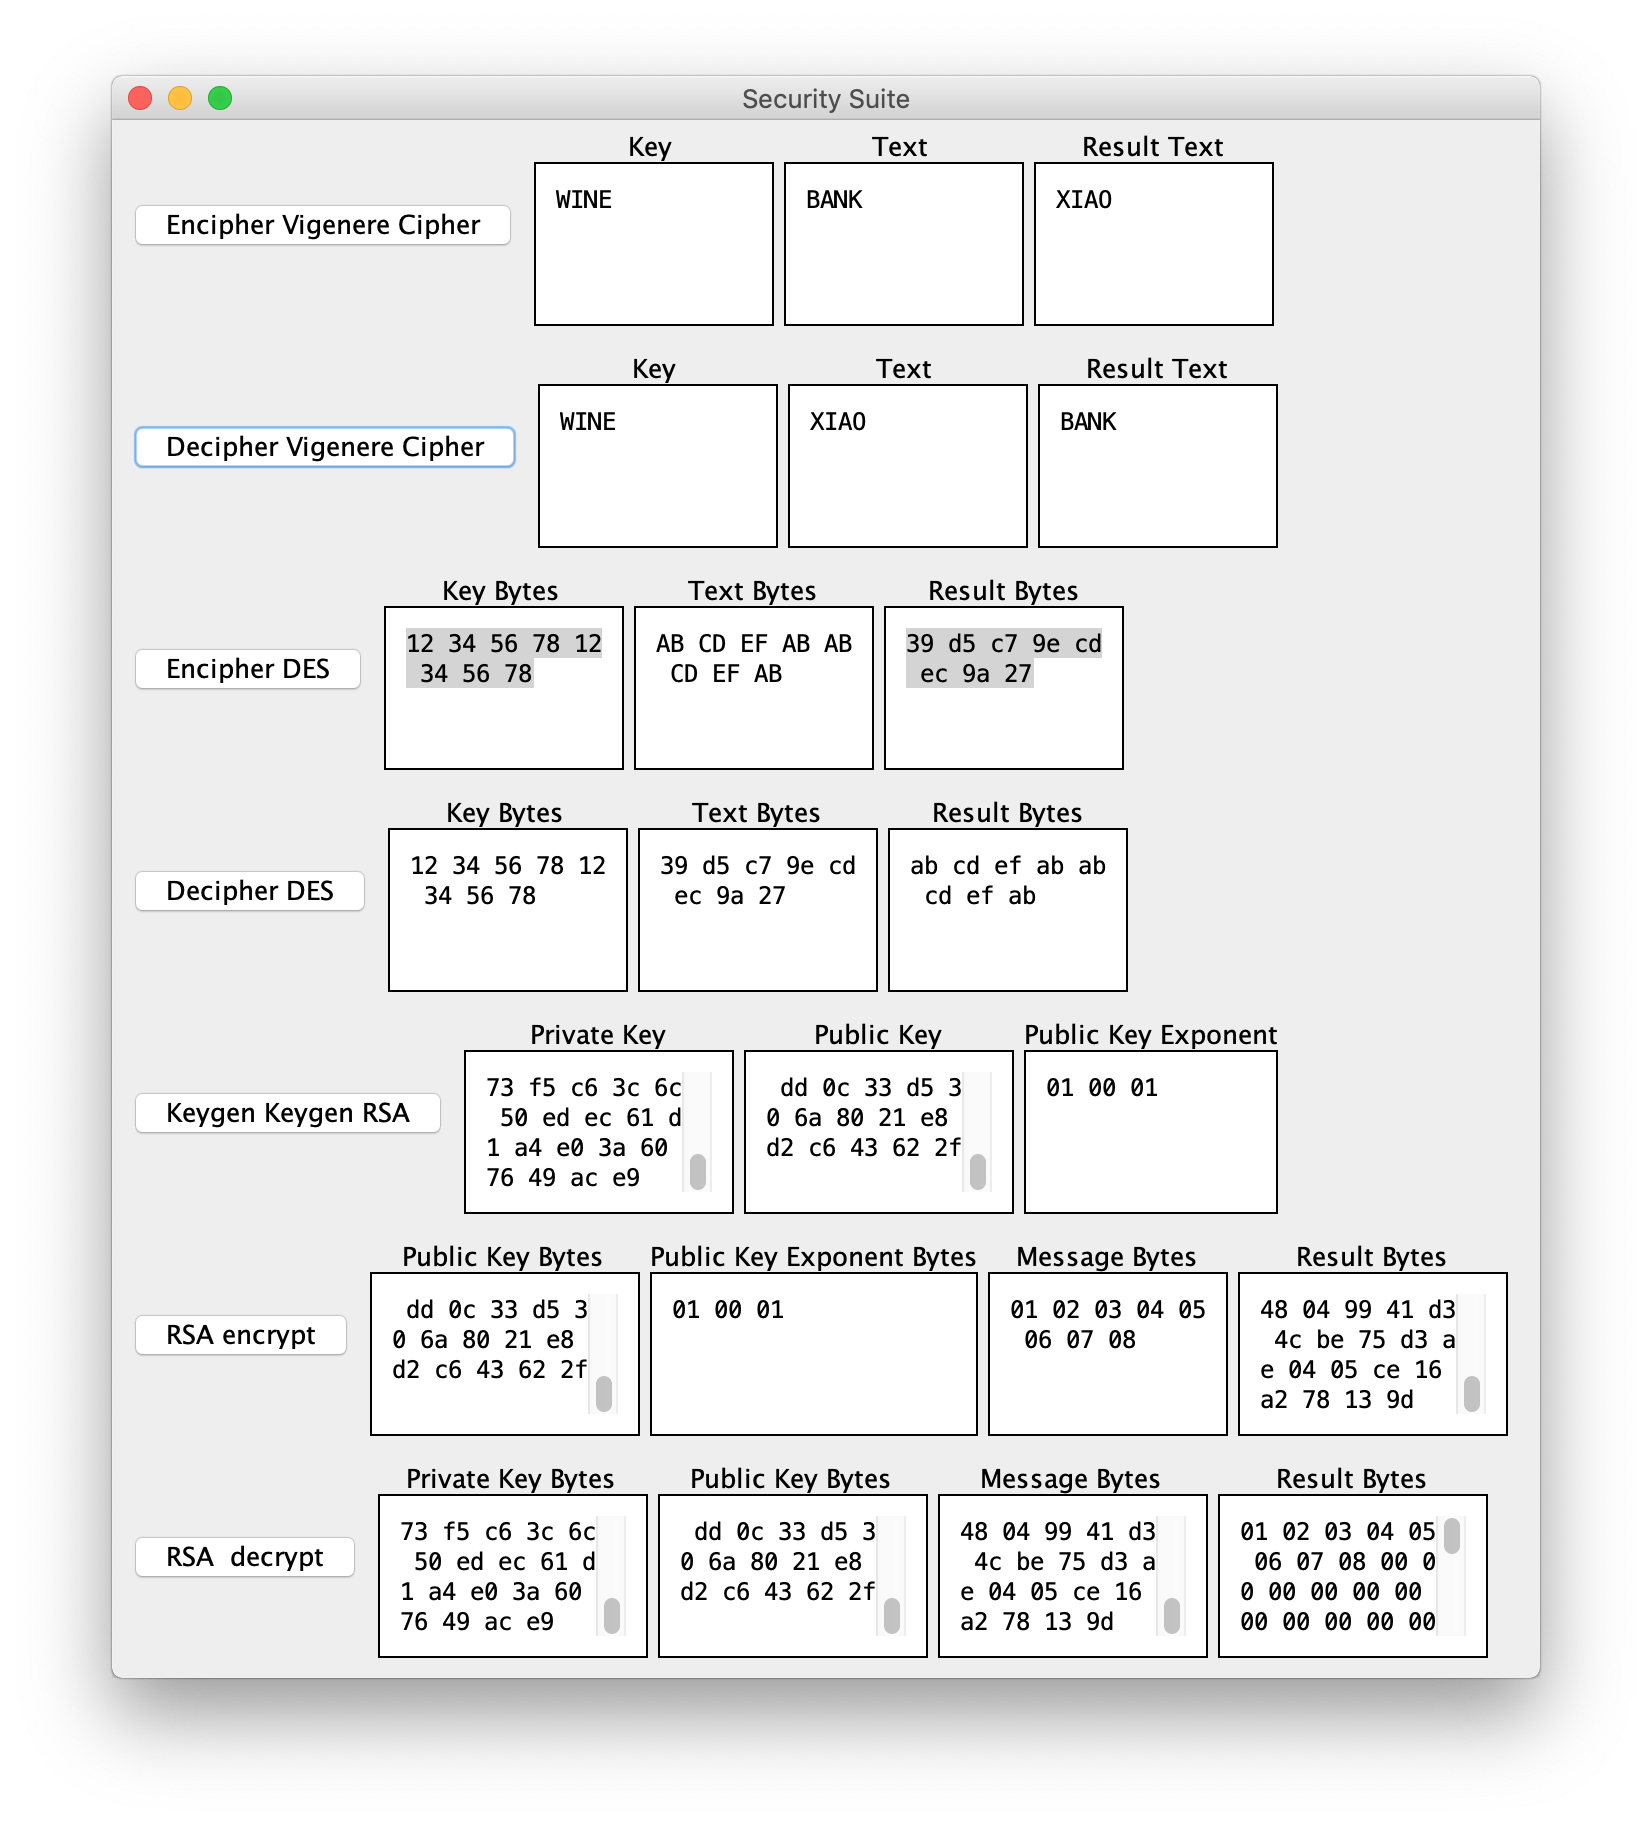
\includegraphics[scale=0.40]{demo}
  \Description{Image of our demo tool}
  \caption{Image of the security suite demo tool.}
  \label{fig:one}
\end{figure}

The GUI (seen in Figure \ref{fig:one}) offers an interface for using all of the algorithms described in the previous sections. For the Vigen\`{e}re cipher, the algorithm operates on characters in an alphabet, so the key and text are both interpreted as such. However the rest of the algorithms operate at a binary level, so everything is interpreted/displayed as hexadecimal (the actual encodings used in practice for the messages are not important for using the algorithms).

Each row corresponds to one algorithm function, all algorithms have inputs on the left and then an output on the right, except for RSA keygen, which has no inputs and 3 outputs which compose a keypair.

The GUI delegates to the implementations, by interpreting the text, and transforming between byte arrays and hexadecimal string encoding where appropriate. For DES, the program invokes python as a separate process using the API specified in the DES section.

\subsection{Hashcat}\label{sec:hashcat}

Hashcat is a software tool used to crack passwords by leveraging the highly-parallelized general purpose computation capabilities of GPU \cite{Hashcat}. hashcat will calculate hashes based on one of several attack modes, and the hashes are automatically checked against the hashes selected to be attacked.

The most important option when using hashcat is the \texttt{hash-type}, which specifies the actual hash algorithm that will be used for the attack. For example, you can choose a simple hash algorithm such as \texttt{"md5"}, or you may choose a composition of algorithms such as \texttt{"sha1(\$salt.sha1(\$pass))"}.

Depending on the algorithm, hashcat may or may not be able to leverage the GPU's capabilities effectively. Some algorithms, such as \texttt{bcrypt} are specifically designed to be difficult to parallelize in GPU hardware. Despite having thousands of cores to parallel computation, the algorithm is bottlenecked by the shared memory bus since the algorithm requires operating on a shared block of memory. Other algorithms, such as \texttt{MD5} are able to be run on the order of \textit{trillions} of time per second on modern hardware setups.

The second required option is an \texttt{attack mode}. The simplest is a \texttt{brute-force attack}, which tries all possible combinations in a given keyspace. For example, a brute-force attack may be done on the following charset:

\begin{center}
\texttt{abcdefghijklmnopqrstuvwxyz0123456789}	
\end{center}

If we use this in conjunction with a password length of $6$, this will try all passwords composed of $6$ characters from that charset. For example, the password \texttt{k39a1j} will be discovered this way.

When trying to crack many passwords, the simple \texttt{brute-force attack} is usually an unrealistic attack method. The \texttt{mask attack} can use multiple charsets and string patterns to reduce the password candidate keyspace.

Hashcat offers many pre-specified charsets to make composing mask attacks easier:

\begin{center}
\begin{minipage}{8cm}
\begin{verbatim}
?l = abcdefghijklmnopqrstuvwxyz
?u = ABCDEFGHIJKLMNOPQRSTUVWXYZ
?d = 0123456789
?h = 0123456789abcdef
?H = 0123456789ABCDEF
?s = «space»!"#$%&'()*+,-./:;<=>?@[\]^_`{|}~
\end{verbatim}
\end{minipage}
\end{center}

For example, it is very common for users to choose passwords that are comprised of lowercase letters followed by numbers. The mask \texttt{?l?l?l?l?d?d} specifies all possible combinations of 4 lowercase letters followed by 2 digits, reducing the search space to $26^410^2$ passwords. A password in this sense would have about 25 bits of entropy (log of the total number of possible passwords).

We can try to build upon knowledge we have about the source of the hash to choose an effective keyspace for an attack. For example, if we know that the website we are trying to attack requires at least one non-alphanumeric symbol in their passwords, then we we would only ever try masks containing at least one \texttt{?s} charset, such as \texttt{?l?l?l?l?s}

Many of these assumptions are based on the idea of a very general, human target. But what if we are only concerned with cracking one single password hash belonging to one individual? In this case, we can try to leverage more information for a targeted attack.

An example of this would be if we knew our target had children, and figured they may use their children's names in their passwords. We can use the \texttt{hybrid attack} mode to combine a dictionary with a mask, for example if our dictionary is \verb|{jim,jane,jack}|, and we use the mask \texttt{?d?d?d}, then we can try all the passwords of the form \texttt{[name][d][d][d]} such as \texttt{jim123}, \texttt{jane032}, and so on. This variation would have a search space to $3^110^3$ passwords (about 12 bits of entropy).

An interesting limitation of many of these methods is the GPU computing platform itself. For example, with a dictionary attack, hashcat can only combine two dictionaries, not three. When doing an attack by combining 3 dictionary words, the CPU must be used, which then becomes the bottleneck. Candidate passwords can be piped from stdout of the separate CPU-powered program into stdin of hashcat.

In the hashcat demo, we explore all of these ideas on some real-world datasets, such as a list of the most commonly-used passwords, and using dictionaries comprised of common English words. We perform many simple attacks that are tractable on a weaker machine, and then leverage an Amazon \textit{EC2 p2.xlarge} instance, with access to a NVIDIA K80 GPU in order to perform an attack requiring a bit more computing power.

\section{Vigen\`{e}re Cipher Cracker}\label{sec:vinegar}

We wrote a Vigen\`{e}re Cipher Cracker using a Ruby script that breaks down the steps needed to find the key for an encoded text. We encoded the first sentence of "A Tale of Two Cities" and used the following steps to determine that "LEMON" was the key used to encode the text.

The first step is to remove all non-letters form the text (such as spaces, punctuation, etc.) and make the text the same case, we chose uppercase.

Then we needed to find the letter position offsets between repeated substrings within the text. We used substrings of size 3 and iterated through the text, finding repeated instances of the substring. Then we subtracted the positions of the beginning letters of the substring occurrences to find the offset and printed them out. The offsets can be used to find the likely length of the key.

We then prompted the user to input their guess for the length of the key. A likely length would be a common factor amongst all or most of the offsets. In our case, a common factor is 5, therefore 5 should be a good guess.

Using the inputted length from the user, we divided the text into chunks of that length and printed out the chunks. For example, if the text was "ABCDEFGHIJK", and the length was 5, "ABCDE FGHIJ K" was printed.

Then we counted the number of times each letter occurred in each position in the 5 letter chunk. Due to 'E' being the most common letter in the English language, we can subtract 'E' from each letter to get the most likely letters in the key. We printed out the top 3 likely letters for each letter position for the key.

Then we found all combinations of letters in each position that could be a possible key and printed them out (243 possible keys). We then deciphered the text using each of the 243 keys and compared the letter frequency of the deciphered text to the actual letter frequency of the English language to find the correlation frequency. After going through each key, we printed out the top 10 correlation frequencies and the keys that corresponded to them. It is very likely the correct key is the one with one of the highest correlation frequencies. In our case, the highest correlation frequency was "LEMON", which was also the correct key.

\section{Results}\label{sec:results}

In our work, we used DES, Vignere, and RSA encrypt and decrypt messages. However, each approach had differing degrees of implementation complexity and confidentiality strength. In DES, the original message had to undergo many stages of modification before returning an encrypted message. Compared to DES, the Vignere cipher was much easier to understand as it performed a set number of rotations for each letter in the original message. In RSA, the key generation step required some understanding of modular arithmetic, but the encryption and decryption steps required a single modular exponentiation. In addition to differing implementation complexities in each cryptographic algorithm, each algorithm also had vulnerabilities or shortcomings. As of current literature, DES is considered unsafe as it is susceptible to cryptanalysis attacks \cite{DESCryptanalysis}. Though AES came to replace DES and is considered secure, AES and DES are both symmetric encryption methods that rely on a secure initial key exchange. Like DES and AES, the Vignere cipher is also a symmetric algorithm and requires the same dependency of a secure initial key exchange. However, as was shown by our Vignere statistical attack tool, Vignere is much more susceptible to attacks than DES and AES. Unlike DES, AES, and Vignere, RSA is an asymmetric cryptographic algorithm that does not rely on a secure initial key exchange. However, RSA relies on the assumption that it is computationally difficult to factor large primes and solve the Discrete Log Problem. 

\section{Related Work}\label{sec:relatedwork}

Related work. Examples of citations with DOIs: \cite{2004:ITE:1009386.1010128, Kirschmer:2010:AEI:1958016.1958018}. Online citations: \cite{TUGInstmem, Thornburg01, CTANacmart}.

\section{Discussion}\label{sec:discussion}

What didn't we cover? :O

% Appendix
\appendix
\section{Elaboration on the ABCD algorithm}

This is an appendix, maybe about some equation
\begin{displaymath}
P=NP
\end{displaymath}

\section{Supplementary Materials}

\subsection{Hashcat materials}

Materials?

\subsection{Tool: Symmetric Ciphers Online }

\href{http://symmetric-ciphers.online-domain-tools.com/}{Link}

\begin{acks}

The authors would like to thank Professor Xiao and the Case Western Reserve EECS Department.

\end{acks}

% Bibliography
\bibliographystyle{ACM-Reference-Format}
\bibliography{bibliography}

\end{document}